\section{Introduction}
\label{sec:introduction}

Model rocketry is a popular hobby that involves the design, construction, and launch of small rockets powered by solid fuel engines.

Even though, at this scale, models are significantly simplified compared to full-scale rockets, they still can be used to study the principles of aerodynamics, propulsion, and flight dynamics.
One of the key parameters that affect the performance of a model rocket is the drag coefficient $C_d$.

The drag coefficient is a dimensionless quantity that characterizes the aerodynamic drag of an object moving through a fluid.
It is defined as the ratio of the drag force acting on the object to the dynamic pressure of the flow around the object.

\begin{equation}
    C_d = \frac{F_d}{\frac{1}{2} \rho v^2 A}
    \label{eq:drag_force}
\end{equation}

The drag coefficient of a model rocket depends mainly (but not only) on its shape, flow conditions, and properties of the fluid.
In general, it cannot be considered a constant value and may vary significantly during the flight of the rocket.

However, for a small model rocket with a 'classical design', it has been observed that the drag coefficient typically ranges between $0.7$ and $0.8$.
This value is based on empirical data and is used as a rule of thumb during the design and analysis phases.

In this project, we aim to analyze the drag coefficient of one of our model rockets using \texttt{Ansys Fluent}, a popular commercial software used for computational fluid dynamics (CFD) simulations.
Due to inexperience with the software and in general the world of simulations, we will have the necessity to make some strong assumptions and simplifications that might affect the accuracy of the results.

At the end of the project, we will try to validate the CFD simulation results against predictions made using another software for model rocket design and simulation, and against actual flight data collected during a previous launch.

The model rocket analyzed in this project is shown in Figure \ref{fig:model_rocket_img}.

\begin{figure}[H]
    \centering
    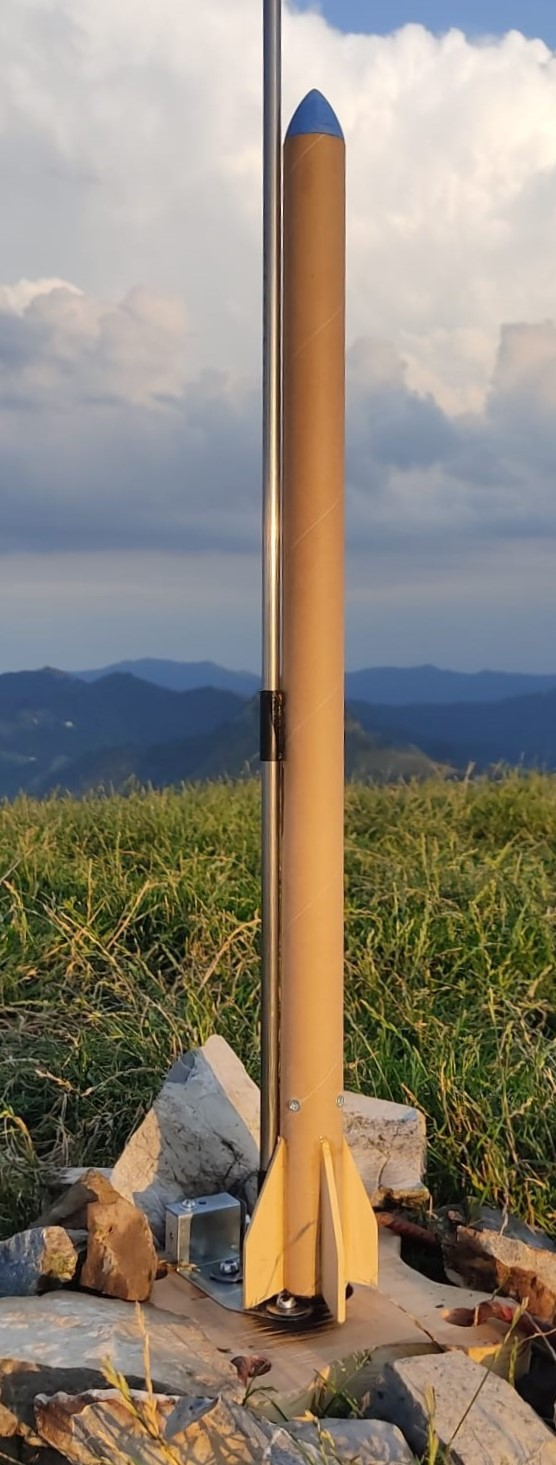
\includegraphics[width=.28\textwidth]{img/Rocket.jpg}
    \caption{Picture of the model rocket analyzed in this project. Photo of the author (July 21, 2023).}
    \label{fig:model_rocket_img}
\end{figure}